% !TEX root = ../main.tex
% File: chapters_part1/chap7_2.tex
% Nội dung cho Chương 7, Phần 2

\section{Các Benchmark Kinh điển và Hiện đại}
\label{sec:benchmarks}

Một metric riêng lẻ chỉ đo lường một khía cạnh của mô hình. Để có một đánh giá toàn diện, cộng đồng nghiên cứu đã tạo ra các \textbf{benchmark} -- những bộ sưu tập các bộ dữ liệu và tác vụ được tiêu chuẩn hóa. Các benchmark đóng vai trò như những "kỳ thi Olympic" cho các mô hình NLP, cho phép các nhà nghiên cứu so sánh một cách công bằng và theo dõi sự tiến bộ của toàn ngành.

Sự phát triển của các benchmark cũng phản ánh sự tiến hóa của chính các mô hình NLP.

\subsection{Kỷ nguyên Pre-LLM: GLUE và SuperGLUE}
\label{ssec:pre_llm_benchmarks}
Trước khi các LLM lớn với khả năng zero-shot ra đời, các mô hình (như BERT) thường được đánh giá bằng cách tinh chỉnh (fine-tune) trên một loạt các tác vụ Hiểu Ngôn ngữ Tự nhiên (NLU) đa dạng. GLUE và SuperGLUE là hai benchmark tiêu biểu nhất cho kỷ nguyên này.

\subsubsection{GLUE: Một Bài kiểm tra Năng lực Ngôn ngữ Tổng quát}
\begin{itemize}
    \item \textbf{Tên đầy đủ:} General Language Understanding Evaluation.
    \item \textbf{Triết lý:} Một mô hình thực sự hiểu ngôn ngữ phải hoạt động tốt trên nhiều loại tác vụ khác nhau, từ suy luận, phân tích cảm xúc, đến nhận dạng sự tương đồng.
    \item \textbf{Cấu trúc:} GLUE bao gồm 9 tác vụ NLU khác nhau, được nhóm thành các loại:
        \begin{itemize}
            \item \textbf{Suy luận Ngôn ngữ Tự nhiên (NLI):} MNLI, QNLI, RTE.
            \item \textbf{Tương đồng Ngữ nghĩa và Diễn giải:} MRPC, QQP, STS-B.
            \item \textbf{Phân loại câu đơn:} SST-2 (cảm xúc), CoLA (tính đúng ngữ pháp).
        \end{itemize}
    \item \textbf{Đánh giá:} Một mô hình được fine-tune riêng cho từng tác vụ. Điểm số cuối cùng là điểm trung bình trên tất cả các tác vụ.
    \item \textbf{Tác động:} GLUE đã trở thành một "thước đo vàng" để đánh giá các mô hình như BERT, RoBERTa. Tuy nhiên, các mô hình nhanh chóng đạt đến và \textbf{vượt qua cả hiệu năng của con người} trên benchmark này vào khoảng năm 2019, cho thấy nó đã trở nên quá "dễ".
\end{itemize}

\subsubsection{SuperGLUE: Nâng cấp Độ khó}
\begin{itemize}
    \item \textbf{Động lực:} Do GLUE đã bị "chinh phục", SuperGLUE được tạo ra với các tác vụ khó hơn, đòi hỏi khả năng suy luận phức tạp hơn.
    \item \textbf{Cấu trúc:} Nó cũng là một bộ sưu tập các tác vụ đa dạng, nhưng tập trung nhiều hơn vào:
        \begin{itemize}
            \item \textbf{Hỏi-đáp yêu cầu suy luận:} BoolQ, MultiRC.
            \item \textbf{Suy luận nhân quả:} COPA.
            \item \textbf{Giải quyết đồng tham chiếu:} WSC.
        \end{itemize}
    \item \textbf{Tác động:} SuperGLUE đã tiếp tục là một thách thức trong một thời gian, nhưng rồi các mô hình lớn hơn cũng dần chinh phục được nó. Sự bão hòa của các benchmark này cho thấy một giới hạn của mô hình fine-tuning và sự cần thiết của các phương pháp đánh giá mới.
\end{itemize}

\subsection{Kỷ nguyên LLM: Đánh giá các Khả năng Nổi trội (Emergent Abilities)}
\label{ssec:llm_benchmarks}
Với sự ra đời của các LLM có khả năng few-shot, mô hình đánh giá đã thay đổi. Thay vì fine-tuning, các benchmark mới tập trung vào việc đo lường kiến thức và khả năng suy luận của mô hình trong cài đặt zero-shot và few-shot.

\subsubsection{MMLU: Bài kiểm tra Kiến thức Đa chuyên ngành}
\begin{itemize}
    \item \textbf{Tên đầy đủ:} Massive Multitask Language Understanding.
    \item \textbf{Triết lý:} Một LLM mạnh phải có kiến thức sâu rộng trên nhiều lĩnh vực chuyên môn, tương tự như các kỳ thi chuẩn hóa của con người.
    \item \textbf{Cấu trúc:} MMLU bao gồm gần 16,000 câu hỏi trắc nghiệm được lấy từ các kỳ thi thực tế, bao phủ 57 môn học khác nhau, từ các môn cơ bản (toán tiểu học) đến các môn chuyên ngành cấp độ đại học và chuyên nghiệp (luật, y, kỹ thuật).
    \item \textbf{Đánh giá:} Các mô hình được đánh giá ở chế độ \textbf{few-shot (thường là 5-shot)}. Prompt sẽ bao gồm 5 câu hỏi và câu trả lời mẫu từ một môn học, sau đó là câu hỏi thực sự cần trả lời.
    \item \textbf{Tác động:} MMLU đã trở thành một trong những benchmark quan trọng nhất để đo lường kiến thức và khả năng suy luận của các LLM hàng đầu. Việc một mô hình đạt điểm cao trên MMLU là một minh chứng mạnh mẽ cho năng lực của nó.
\end{itemize}

\subsubsection{Big-Bench: Khám phá Giới hạn của LLMs}
\begin{itemize}
    \item \textbf{Tên đầy đủ:} Beyond the Imitation Game benchmark.
    \item \textbf{Triết lý:} Các benchmark hiện có vẫn còn hạn chế. Chúng ta cần một bộ sưu tập các tác vụ cực kỳ đa dạng và sáng tạo để thăm dò các khả năng và những điểm yếu bất ngờ của LLM.
    \item \textbf{Cấu trúc:} Một sự hợp tác khổng lồ của cộng đồng, tạo ra hơn 200 tác vụ rất đa dạng, bao gồm logic, lý luận toán học, hiểu biết vật lý trực quan, nhận biết định kiến xã hội, và nhiều tác vụ sáng tạo khác mà máy tính trước đây chưa từng làm tốt.
    \item \textbf{Đánh giá:} Chủ yếu ở chế độ \textbf{zero-shot}, để kiểm tra khả năng giải quyết vấn đề "ngay từ đầu" của mô hình.
    \item \textbf{Tác động:} Big-Bench đã giúp các nhà nghiên cứu xác định được các "khả năng nổi trội" (emergent abilities) -- các khả năng chỉ xuất hiện khi mô hình đạt đến một quy mô đủ lớn.
\end{itemize}

\subsubsection{HumanEval: Đánh giá Năng lực Sinh mã nguồn}
\begin{itemize}
    \item \textbf{Dùng cho tác vụ nào?} Đánh giá khả năng \textbf{viết và hoàn thiện mã nguồn (code generation)} của LLM.
    \item \textbf{Cấu trúc:} Bao gồm 164 bài toán lập trình. Mỗi bài toán được đưa ra dưới dạng một docstring (mô tả hàm) và một vài test case.
    \item \textbf{Đánh giá:} Mô hình được yêu cầu sinh ra phần thân của hàm. Mã nguồn được sinh ra sau đó sẽ được thực thi và kiểm tra xem nó có vượt qua được các test case hay không. Metric chính là \textbf{Pass@k}, tức là xác suất một giải pháp đúng được tạo ra trong $k$ lần thử.
    \item \textbf{Tác động:} HumanEval đã trở thành một tiêu chuẩn để đo lường năng lực lập trình của các mô hình như Codex, AlphaCode, và các LLM hiện đại khác.
\end{itemize}

\begin{center}
    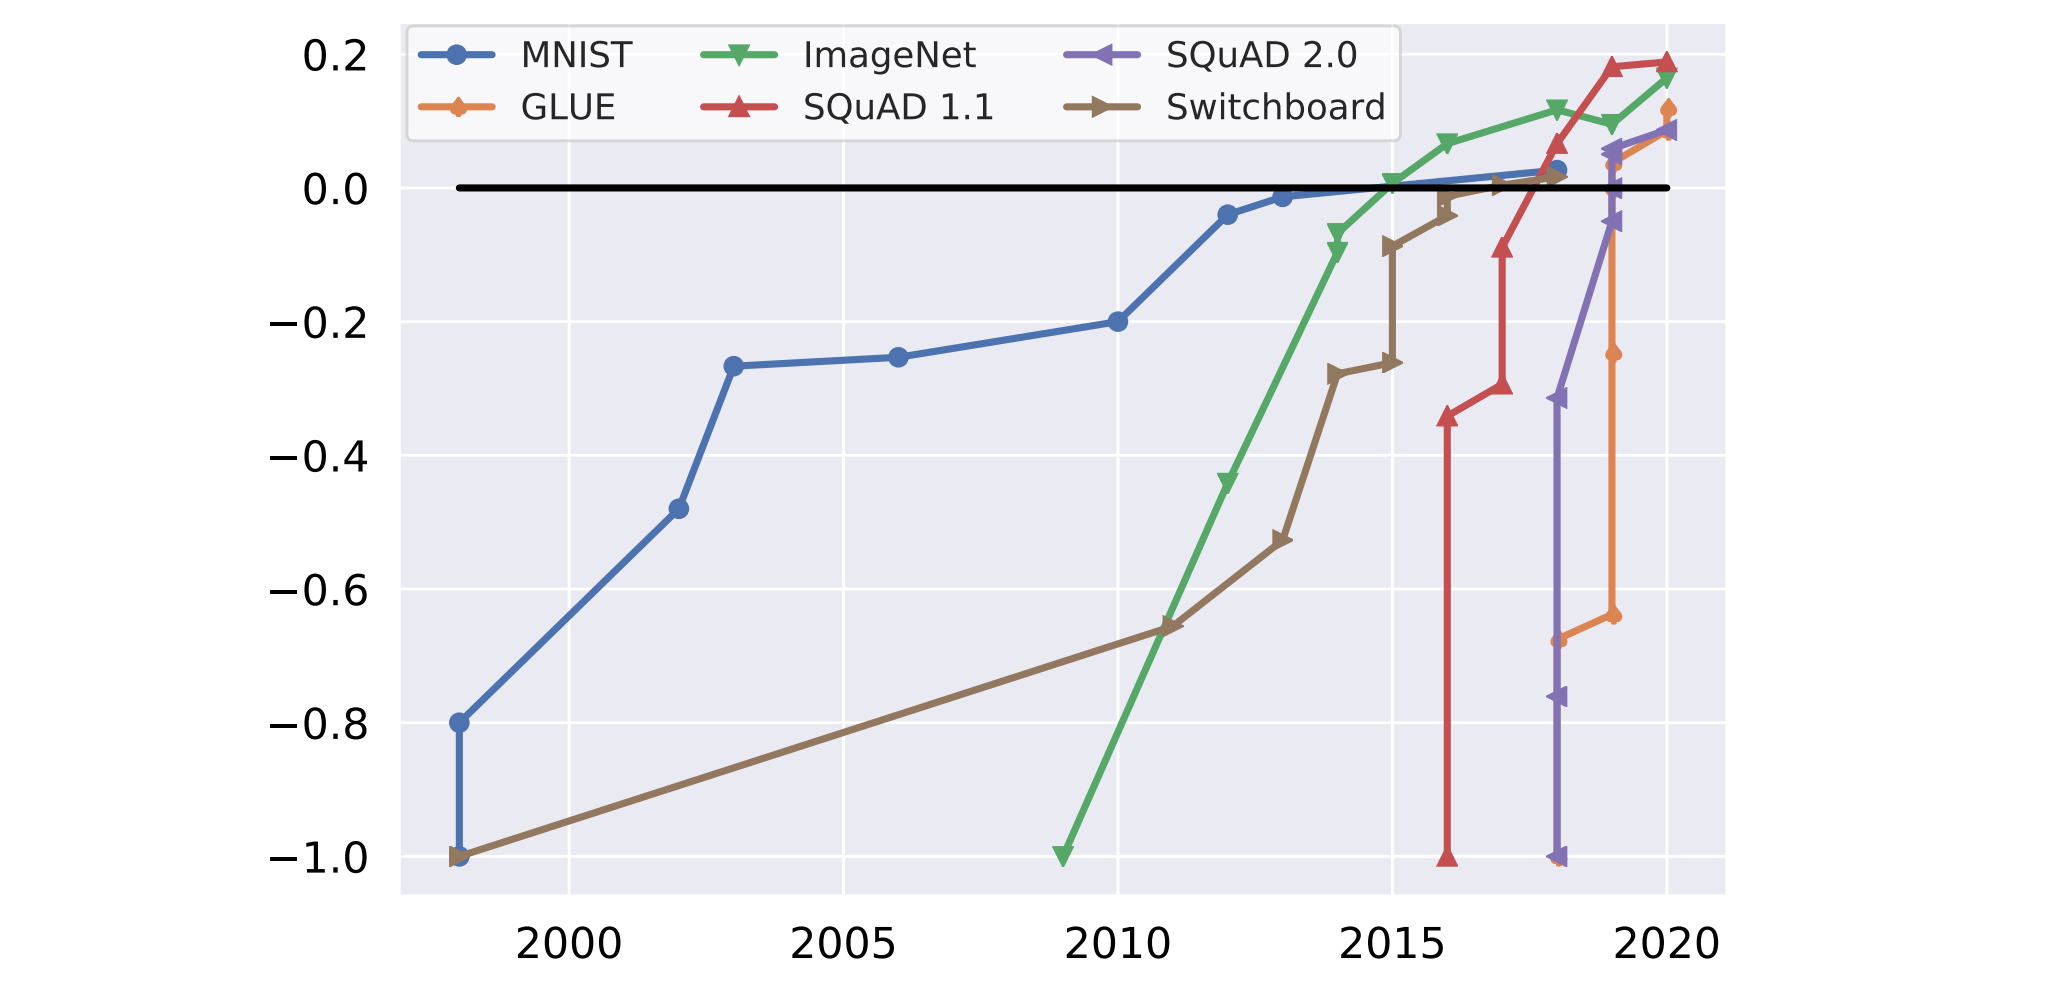
\includegraphics[width=1.0\textwidth]{llm_benchmarks_timeline.png}
    \captionof{figure}{Sơ đồ thời gian thể hiện sự phát triển của các benchmark}
    \label{fig:llm_benchmarks_timeline}
\end{center}

Việc chuyển từ các benchmark như GLUE sang MMLU/Big-Bench không chỉ là một sự thay đổi về quy mô, mà còn là một sự thay đổi cơ bản trong cách chúng ta hiểu và đo lường "trí thông minh" của các mô hình ngôn ngữ.